\documentclass{article}
\usepackage{amsmath}
\usepackage{braket}
\usepackage{amssymb}
\usepackage{hyperref}
\usepackage{booktabs}
\usepackage{graphicx}
\newcommand{\bfit}[1]{\textit{\textbf{#1}}}
\begin{document}
\hfill \textbf{\Large Part II}\\

\hfill \textbf{\Large Silicon Spin Qubit Architecture}

\hfill \textbf{\Large and Hardware}

\newpage
\textbf{\Large
Chapter 7\\
Spin Qubit-Preliminary Physics}\\\\\\
\textbf{\large 7.1 Introduction}\\\\
Spin can be very difficult and confusing concept. Mathematically, spin can 
only be derived in relativistic quantum mechanics (i.e., \textit{quantum electrodynamics. QED}).
The word "relativistic" means that it applies to particles at high velocity, too.
In QED, \textit{Dirac equation} (a relativisitc version form of Schr\"{o}dinger equation)
is used and the concept of spin of an electron appears naturally. In this book,
we will treat spin as a given property of a particle. Indeed, in non-relativistic
quantum mechanics, we take this for granted and we have been treating spin as an
\textit{intrinsic} property of a particle. However, its relationship to angular momentum and magnetic
moment and it interaction with magnetic field need to be clarified to enfance our understanding
and prepare us for more advanced studies in the future.\\\\\\
\bfit{\large 7.1.1 Learning Outcomes}\\\\
Appreciate the gyromagnetic ratio difference in classical and quantum physics;
understand the concept of magnetic moment and angular momentum; understand
the interaction between the magnetic field and a spin angular momentum; be aware
of the effect of the sign of the charge on the value of angular ommentum and spin.\\\\\\
\bfit{\large 7.1.2 Teaching Videos}\\\\

$\bullet$ Seacrh for Ch7 in this playlist

- \url{https://tinyurl.com/3yhze3jn}
\\\\
$\bullet$ Other videos

- \url{https://youtu.be/8Q6XWXVO_6s}\\\\\\
\textbf{\large 7.2 Magnetic Moment, Angular Momentum, and Gyromagnetic Ratio}\\\\
Consider Fig. 7.1 in which a charged particle with a charge $q$ moves along
a circle with radius \bfit{R}, about the origin at velocity $\vec{v}$. In classical
mechanics, it \textbf{angular mementum}, $\vec{L}$, is given by,
\begin{align*}\label{eq 7.1}
    \vec{L}&=\vec{r}\times\vec{p},\\
    &=m\vec{r}\times\vec{v},\tag{7.1}
\end{align*}
where $m,\: \vec{r},$ and $\vec{p}$ are the mass, position, and linear momentum of the
particle, respectively. Let us only consider the case when th eparticel ismoving at a constat speed, $v=\vec{v}$. Since it is moving in a circle, then 
$\vec{v}$ is always perpendicular to $\vec{r}$ and $\vec{r}=R$. Due to the right-hand rule, which can be used to guide the direction 
of a cross-product, we know that the direction of $\vec{L}$ is in the $\hat{z}$ direction. Therefore, we have $m\vec{r}\times\vec{v}=m|\vec{r}|v\sin{90\deg}\hat{z}
=mvR\hat{z}$, which is constant in both magnitude and direction. Therefore,
\begin{equation} \label{eq 7.2}
    \vec{L}=mvR\hat{z},\tag{7.2}
\end{equation}


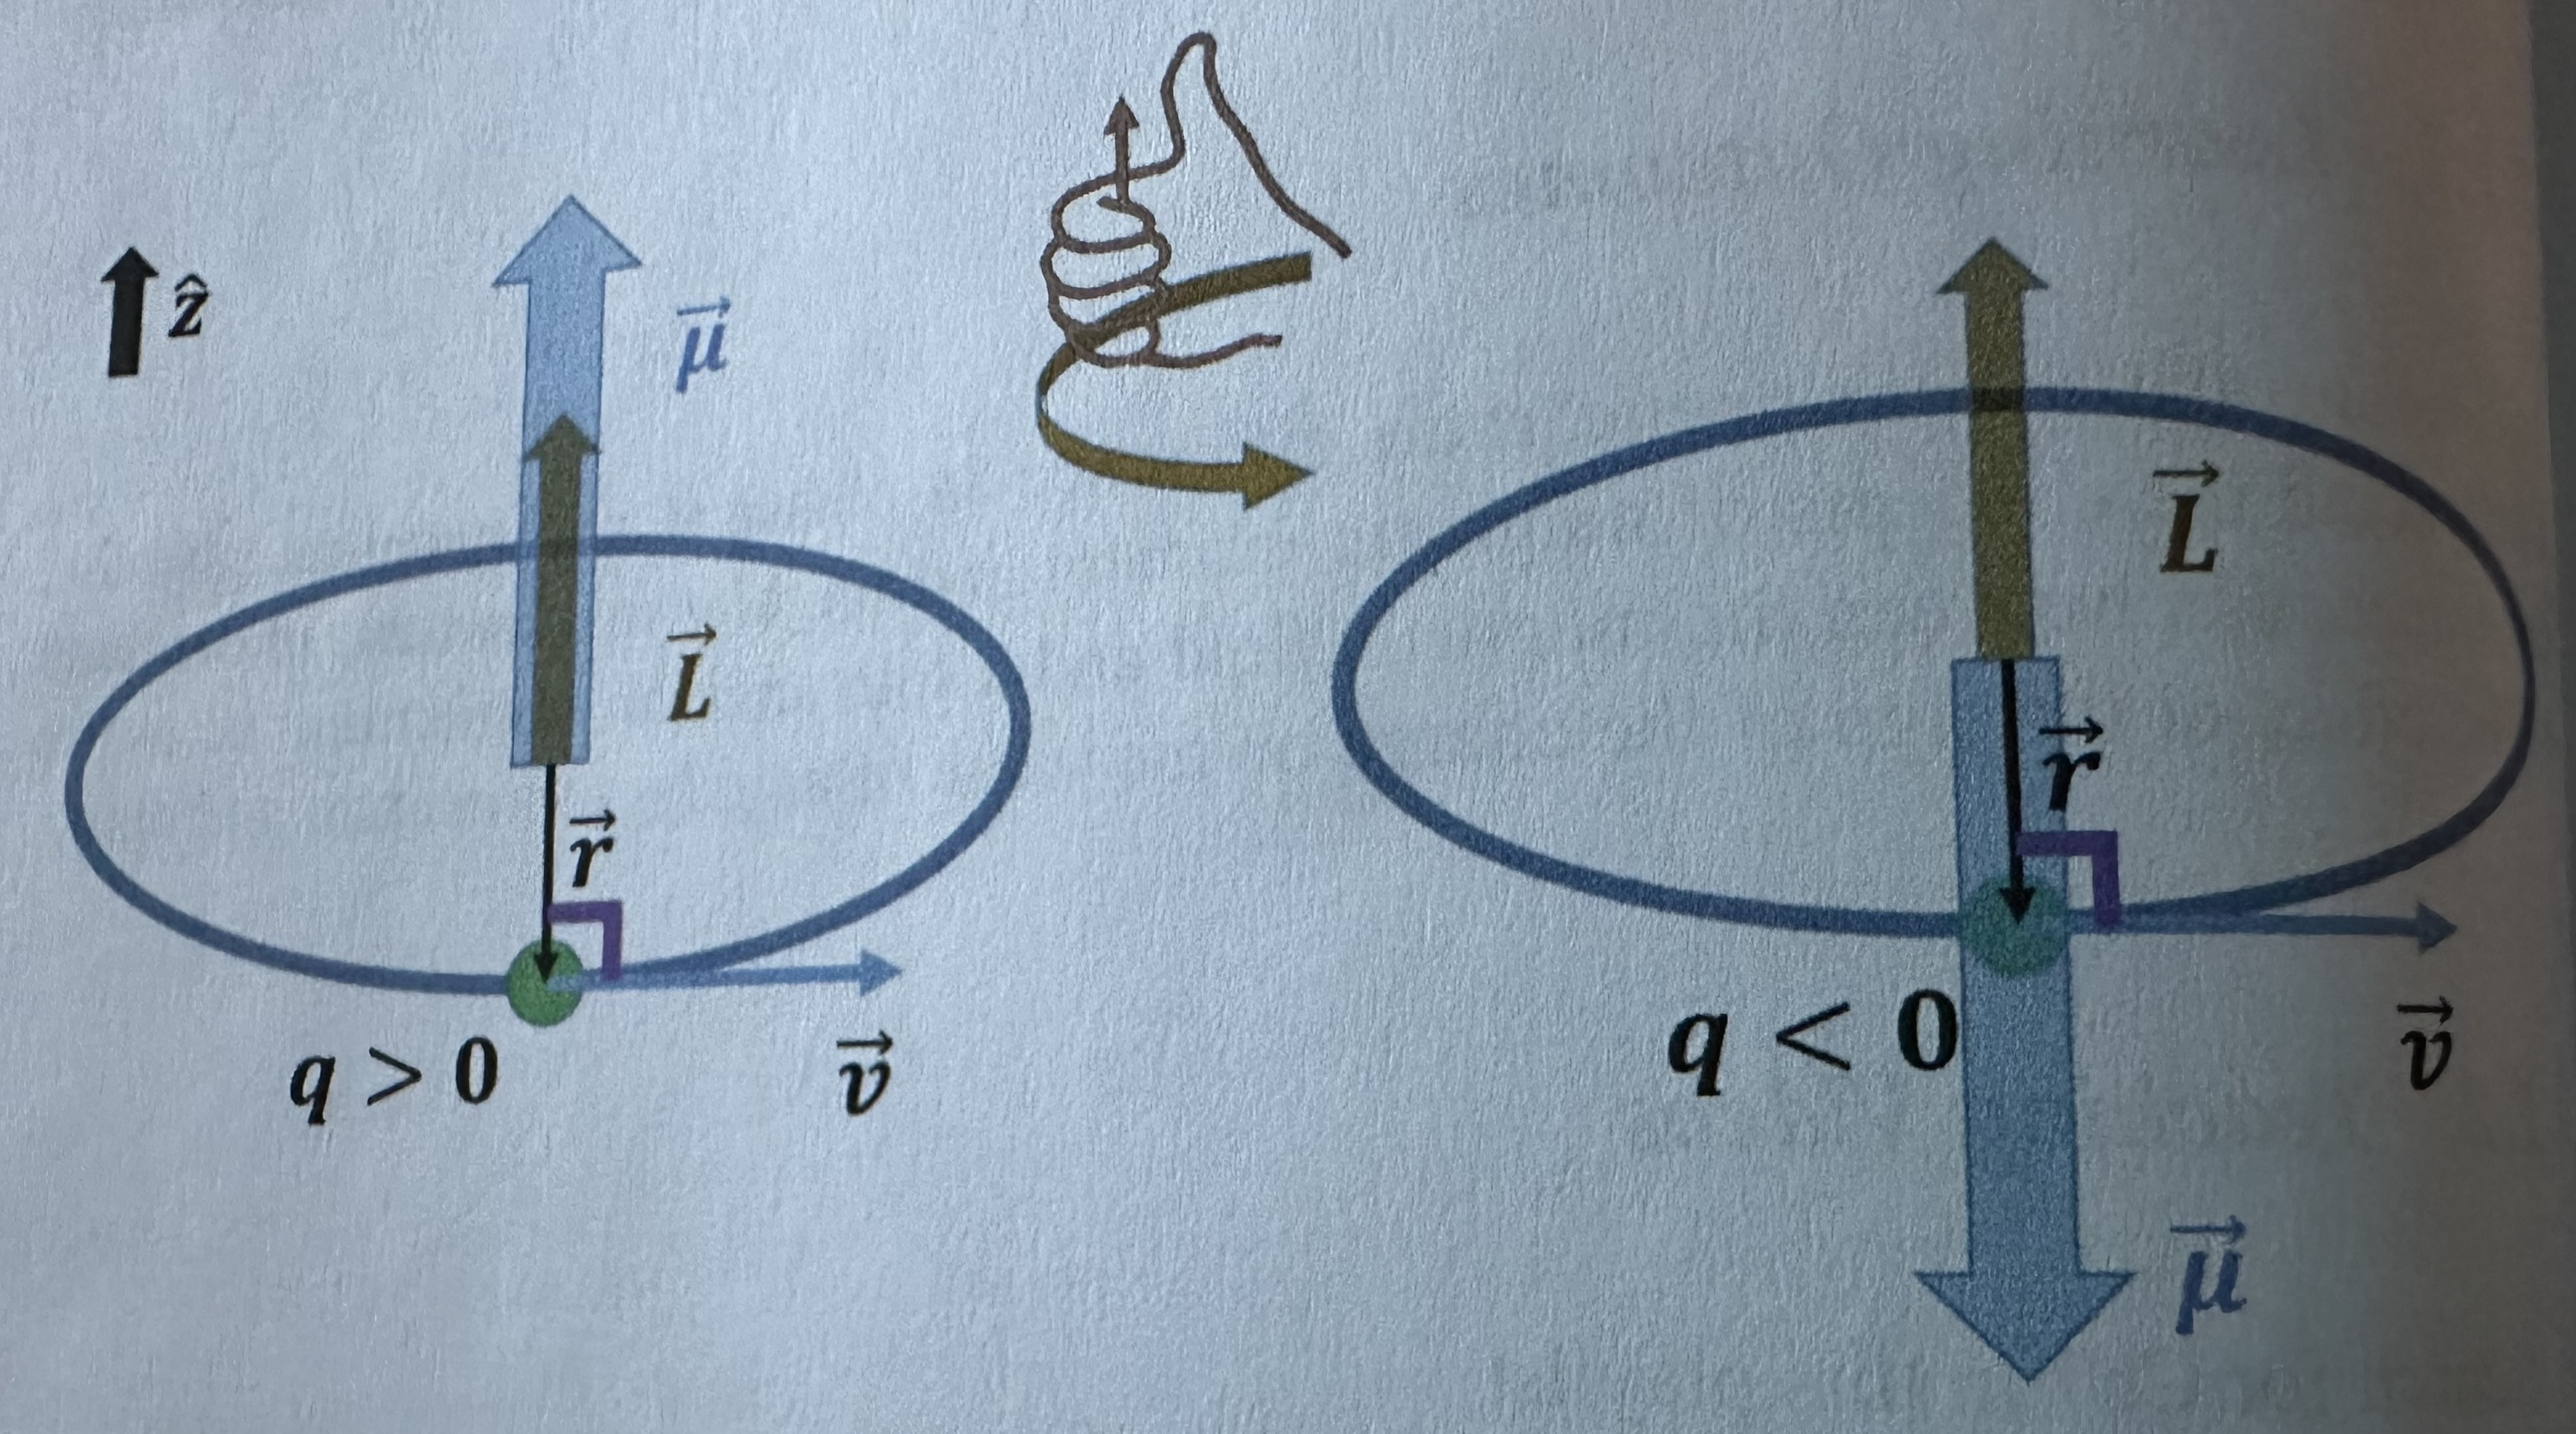
\includegraphics[scale=0.4]{Fig.7.1.jpeg} \\\\
\textbf{Fig. 7.1} Relationship between the angular mementum and the magnetic moment of a charged particle (Left: 
positibe charge. Right: negative charge.) The inset shows the right-hand rule\\\\

A moving charge forms a current, $I$. the current through a cross section is defined as 
the amount of charge passing through that corss section in a unit of time.
Note that the cross section is perpendicular to the path of the particle. In Fig.7.1 the cross
section cuts the circle circumference. The cross section is \textit{not} the circle drawn. Therefore,
\begin{align*}\label{eq 7.3}
    I&=\frac{q}{2\pi R/v},\\
    &=\frac{qv}{2\pi R}, \tag{7.3}
\end{align*}
where $2\pi R/v$ is the amount of time the particle spends to ravel through the circumference
of the circle.

In classical electromagnetism, it is known that a circulating current, $I$, along a
closed path enclosing an area A creates a \textbf{magnetic moment}, $\vec{\mu}$, An
\textbf{area vector}, $\vec{A}$, is defined as a vector with a magnitude A and a direction following
the right-hand ruel for the circulating current. The resulting magnetic moment has a magnitude
of \textit{I A} and a direction the same as $\vec{A}$. Therefore, in our case (left of Fig.7.1),
if the charge is positive and circulating counterclockwise, the current is also following
counterclockwise and
\begin{align*}\label{eq 7.4}
    \vec{\mu}&=I\vec{A},\\
    &=I A \hat{z},\\
    &=I \pi R^2\hat{z},\\
    &=\frac{qv}{2\pi R}\pi R^2\hat{z},\\
    &=\frac{qvR}{2}\hat{z}, \tag{7.4}
\end{align*} 
where we used the fact that $A=\pi R^2$ for a circle in line 3 and Eq. (\ref{eq 7.3})
in line 4.

Now we will derive the relationship between $\vec{\mu}$ and $\vec{L}$ by rearranging Eq. (\ref{eq 7.2})
to be $\frac{\vec{L}}{m}=vR\hat{z}$ and substitute it into Eq. (\ref{eq 7.4}) to obtain,
\begin{align*}\label{eq 7.5}
    \vec{\mu}&=\frac{qvR}{2}\hat{z},\\
    &=\frac{q\vec{L}}{2m},\\
    &=\gamma\vec{L},\tag{7.5}
\end{align*}
where $\gamma=\frac{q}{2m}$ is the \textbf{gyromagnetic ratio} of the particle.
Since $\gamma=\frac{q}{2m}$ and the mass of a particle must be positive,
$\gamma$ is positive (negative) if the charge is positive (negative). $\gamma$
relates the angular momentumm, $\vec{L}$, of a moving charged particle in a 
circle to the magnetic moment, $\vec{\mu}$, it generates. $\vec{L}$ is parallel (anti-parallel)
to $\vec{\mu}$ if the charge is positive (negative).

\textit{If you are not interested in mathematics. I hope you can at least appreciate this.
A moving charged particle has an angular momentum and also generates a magnetic moment.
They are related through the gyromagnetic ratio in Eq.(\ref{eq 7.5})}.\\\\\\
\textbf{\large 7.3 Spin, Spin Angular Momentum, and Spin Magnetic Moment}\\\\
With the classical description of angular magnetic moment and angular momentum
described in the previous section, we will now discuss \textbf{spin, spin angular momentum,}
and \textbf{spin magnetic moment}.

As discussed in Sect. 7.1 spin is an intrinsic property of an elementary particle
(such as an electron and a proton). This is just like the fact that the charge is an
intrinsic property of a particle. This is the safest way to understand spin.
It is wrong to attempt to think of the spin of an elementary particle as the "spinning"
of a ball. The reason is because\textit{it is not}. If you have heard about the \textit{color} of quarks
and you accept that the color of a quark is its intrinsic property and is not the "color"
we see with our eyes, then there is no difficulty in understanding that the spin
is also an intrinsic property.

However, we understand Physics based on our daily lives. While and electron is not spinning,
it has the properties of a spinning ball. First of all, an electron or a proton has the intrinsic property,
called \textit{spin}. In qunatum mechanics, we say that it has a \textbf{spin qunatum number}, $S$, of either
$+\frac{1}{2}$ or $-\frac{1}{2}$. That is
\begin{equation}\label{eq 7.6}
    S=\pm\frac{1}{2}.\tag{7.6} 
\end{equation}

This is given by QED. Note that it only has two possible values because
\textit{we limit ourselves in the discussion of \textbf{spin-half} particles, such as 
electrons and protons}. \textbf{We will only limit to the discussion of electrons}
from now on. We may think of the two values corresponding to spinning clockwise and 
anti-clockwise, respectively. This is wrong but this is a convenient way to link
it to our daily experience. But do not do that if you feel comfortable accepting that the intrinsic
property of an electron can only have two possible values.

Due to spin, it also has an associated spin angular momentum, $\vec{S}$,
\begin{equation}\label{eq 7.7}
    \vec{S}=S\hbar\hat{z}, \tag{7.7}
\end{equation}
which is a vector like the classical angualr momentum and is arbitrarily chosen to be along 
the $\hat{z}$ direction (parallel or anti-paralle depending on S). Since a spinning ball has
non-zero spin angular momentum, it is natural to expect an electron to have an angular momentum,
it is natural to expect an electron to have an angular momentum due to spinm even
though it spin is not the classical "spin".

In Eq.(\ref{eq 7.5}), it is shown that a moving charged particle generates a magnetic
moment that is correlated to its angular momentum of an electron will also generate a spin
magnetic moment, $\vec{\mu_e}$, and they are related through the gyromagnetic ratio,
\begin{equation}\label{eq 7.8}
    \vec{\mu_e}=\gamma\vec{S}. \tag{7.8}
\end{equation}

However, there is an important difference from the classical case. The $\gamma$ of spin
is about 2.002 times of they $\gamma$ of the classical case for an electron. Note that an electron
has a negative charge of $q=-e=-1.6\times10^{-19}C$. Therefore, Eq. (\ref{eq 7.5}) becomes
$\gamma\approx -2.002\frac{e}{2m}$. We now introduce a new term called the \textbf{g-factor}, 
g, which is about -2.002 to account for the difference. Equation (\ref{eq 7.8}) becomes
\begin{align*}\label{eq 7.9}
    \vec{\mu_e}&=g\frac{e}{2m}\vec{S},\\
    &=g\frac{e\hbar}{2m}\frac{\vec{S}}{\hbar},\\
    &=g\mu_B\frac{\vec{S}}{\hbar}, \tag{7.9}
\end{align*}
where \textbf{Bohr magnetron}, $\mu_B=\frac{e\hbar}{2m}$, is introduced. This is approximately
the magentic moment an electron particel has due to its spin (as $|\frac{g\vec{S}}{\hbar}|\approx 1$).

In summary, the gyromagnetic ratio of an electron is about $\frac{-e}{m}$, which is negative
as in the classical case. The means that if an electron has a spin angualr momentum in the positive
direction, $\vec{S}=\frac{\hbar}{2}\hat{z}$ (or positive spin, $S= +\frac{1}{2}$), it has a spin magnetic moment,
$\vec{\mu_e}$, in the negative driection and vice versa. This is shown on the right of Fig.7.2.\\

\begin{center}
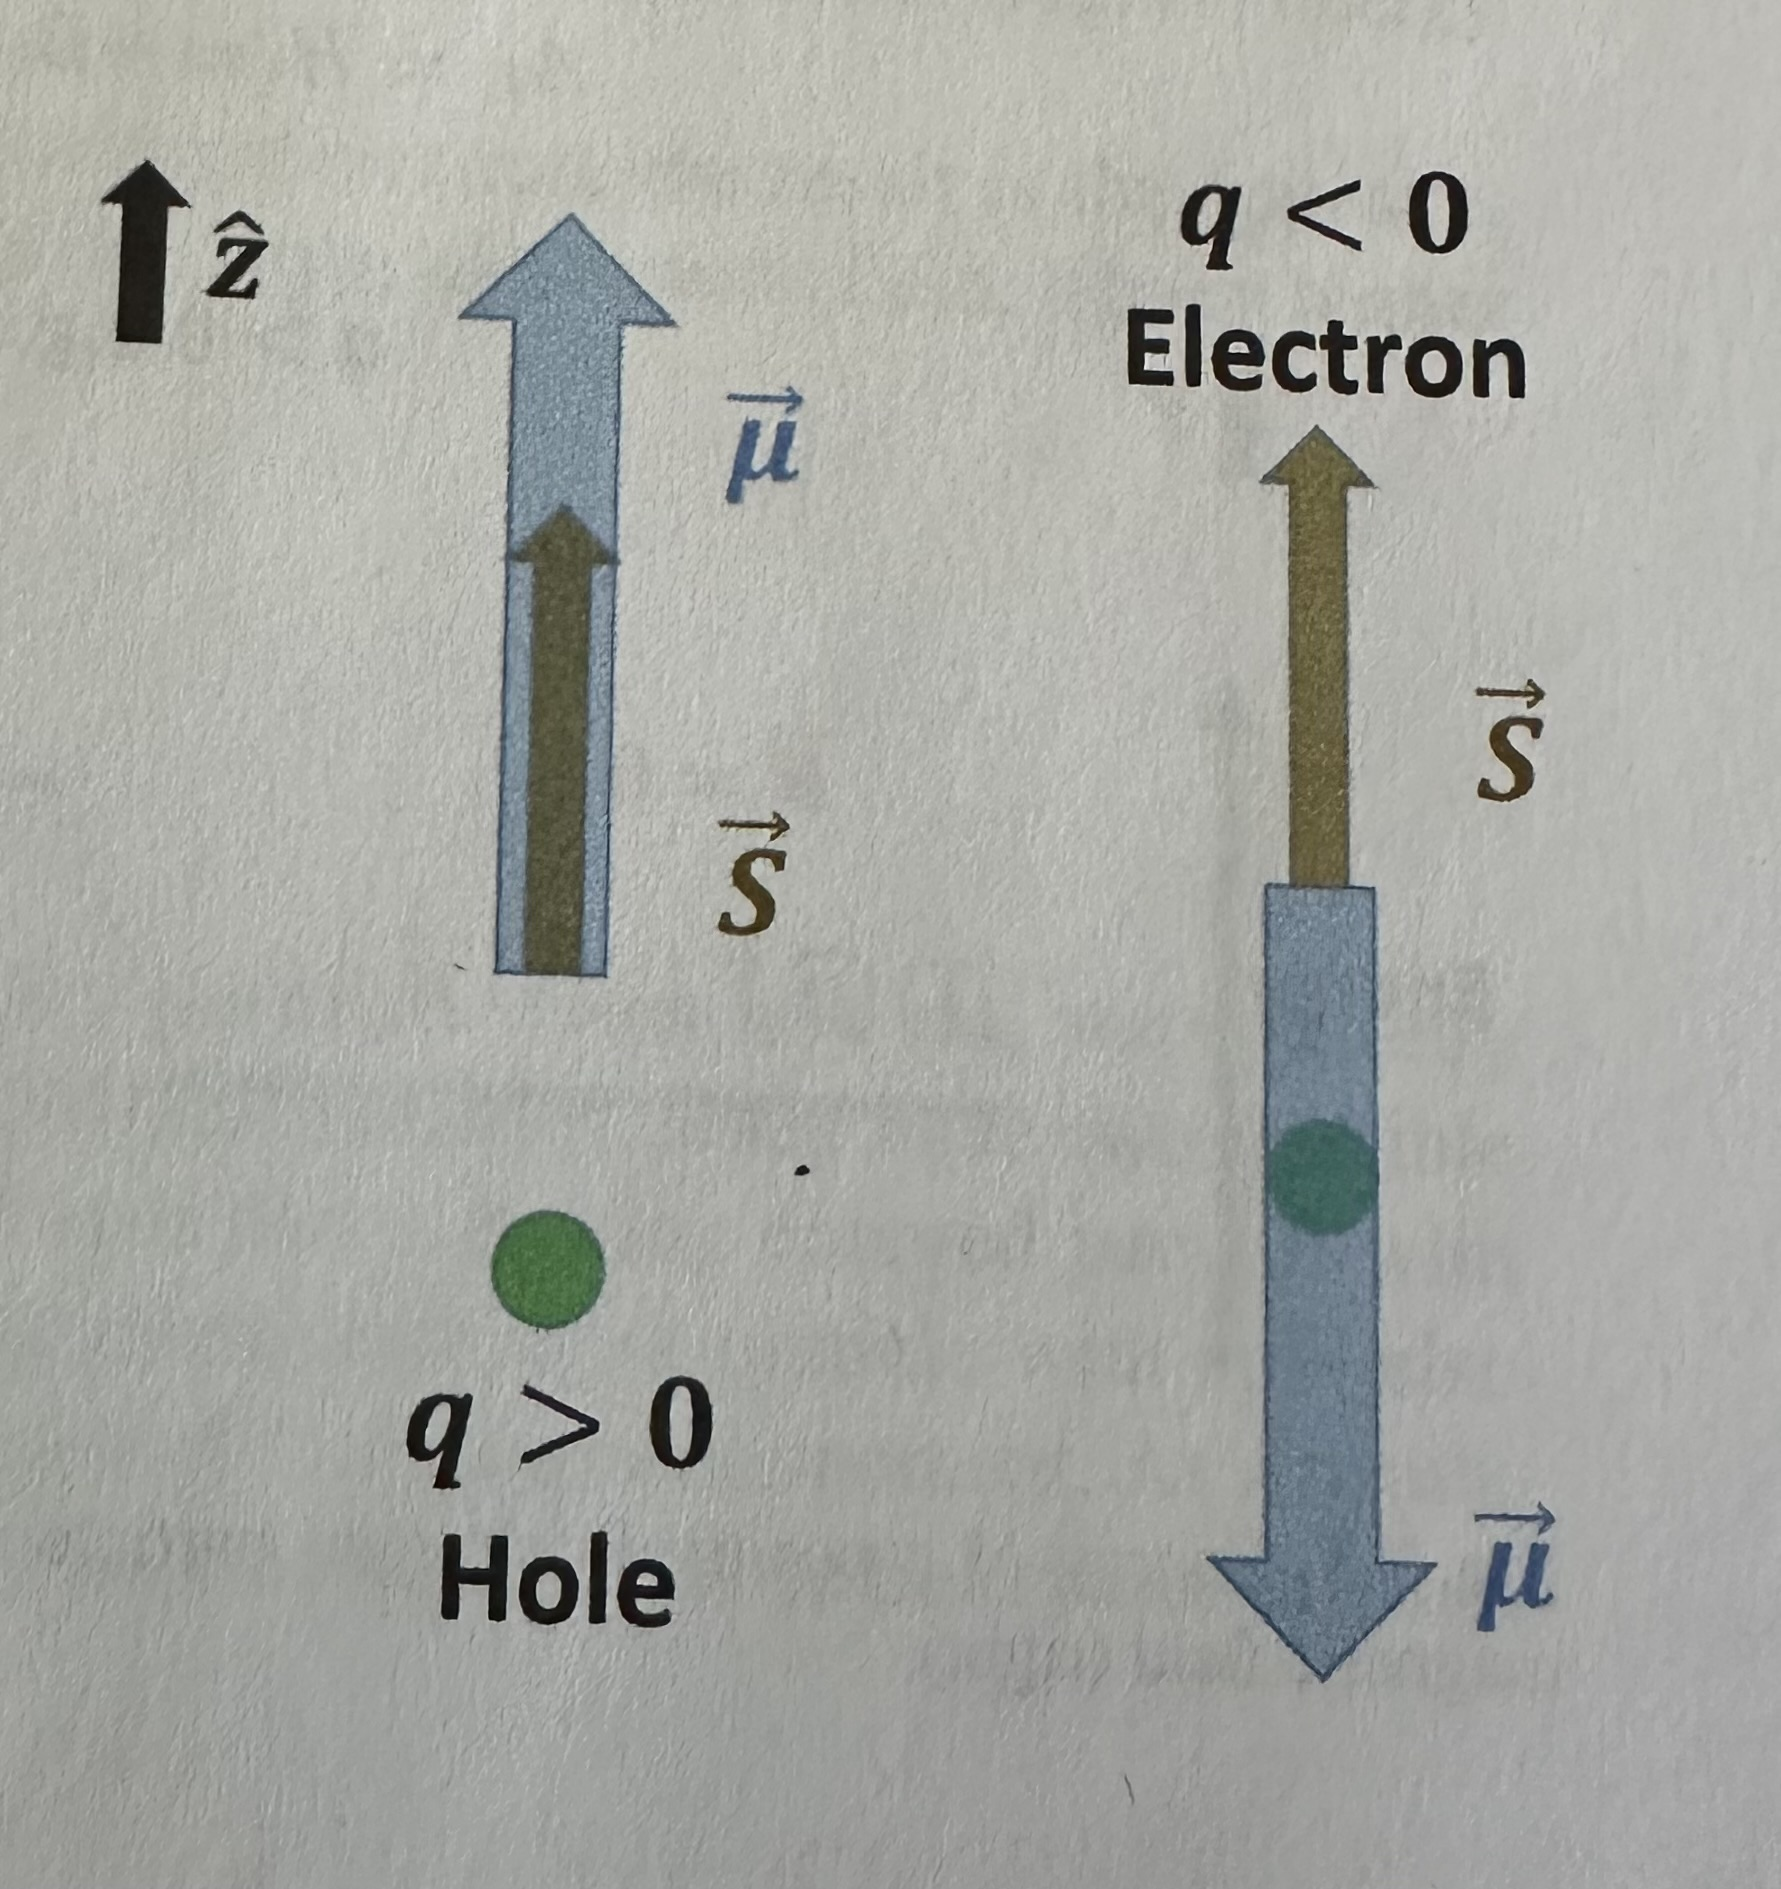
\includegraphics[scale =0.4]{Fig. 7.2.jpeg}\\    
\end{center}
\textbf{Fig. 7.2} relationship between the spin angular momentum and the spin magnetic moment of a charged particel of a hole
(left) and an electon (right)\\

To prepare for future discussion, a \textbf{hole} (lack of an electron) in a semiconductor
is also spin-half. Its spin magnetic moment has the same direction as its spin angular momentum
(left of Fig. 7.2) due to its positive charge.\\\\\\
\textbf{\large 7.4 Intecation Between MAgnetic Moment and an External Magnetic Field}\\\\
How do we know if an electron ($q=-e<0$) or a hole ($q=e>0$) spins up,
$\ket{\uparrow}$ or $S=\frac{1}{2}$, or spins down, $\ket{\downarrow}$? We do not know until
we do a measurement. While we can look at a bail to determine if it is spinning clockwise or
 counterclockwise, we cannot measure the spin of an elementary particle in the same way.
This is because spin is an intrinsic property of an elementary particle and it is not a 
mechanical spin. We can try to measure its energy if different spin states have different energies.

However, if there is no external magnetic field, both states are indistinguishable
(left of Fig. 7.3). In other words, an electron or a hole has the same energy in both states
in the absence of a magnetic field. This is easy to understand. When there is no external magnetic field, 
the space is the same (imagine we are floating in an empty universe). So it is natural for a particel to have
same energy regardless of its spin. This is called \textbf{degeneracy} and both states
are \textbf{degenerated states}.

When there is an external magnetic field, $\vec{B}$, the space is nolonger isotropic for this
particle. This is because the spin magnetic moment interacts with the magnetic field,
resulting in different energies in different spin states. We say that the \textit{degeneracy is lifted}.
The change if energy due to the magnetic field. $\Delta_E$, is given by 
\begin{align*}\label{eq 7.10}
    \Delta_E&=H=-\vec{B}\cdot\vec{\mu},\\
    &=-|\vec{B}||\vec{\mu}|\cos{\theta},\tag{7.10}
\end{align*}

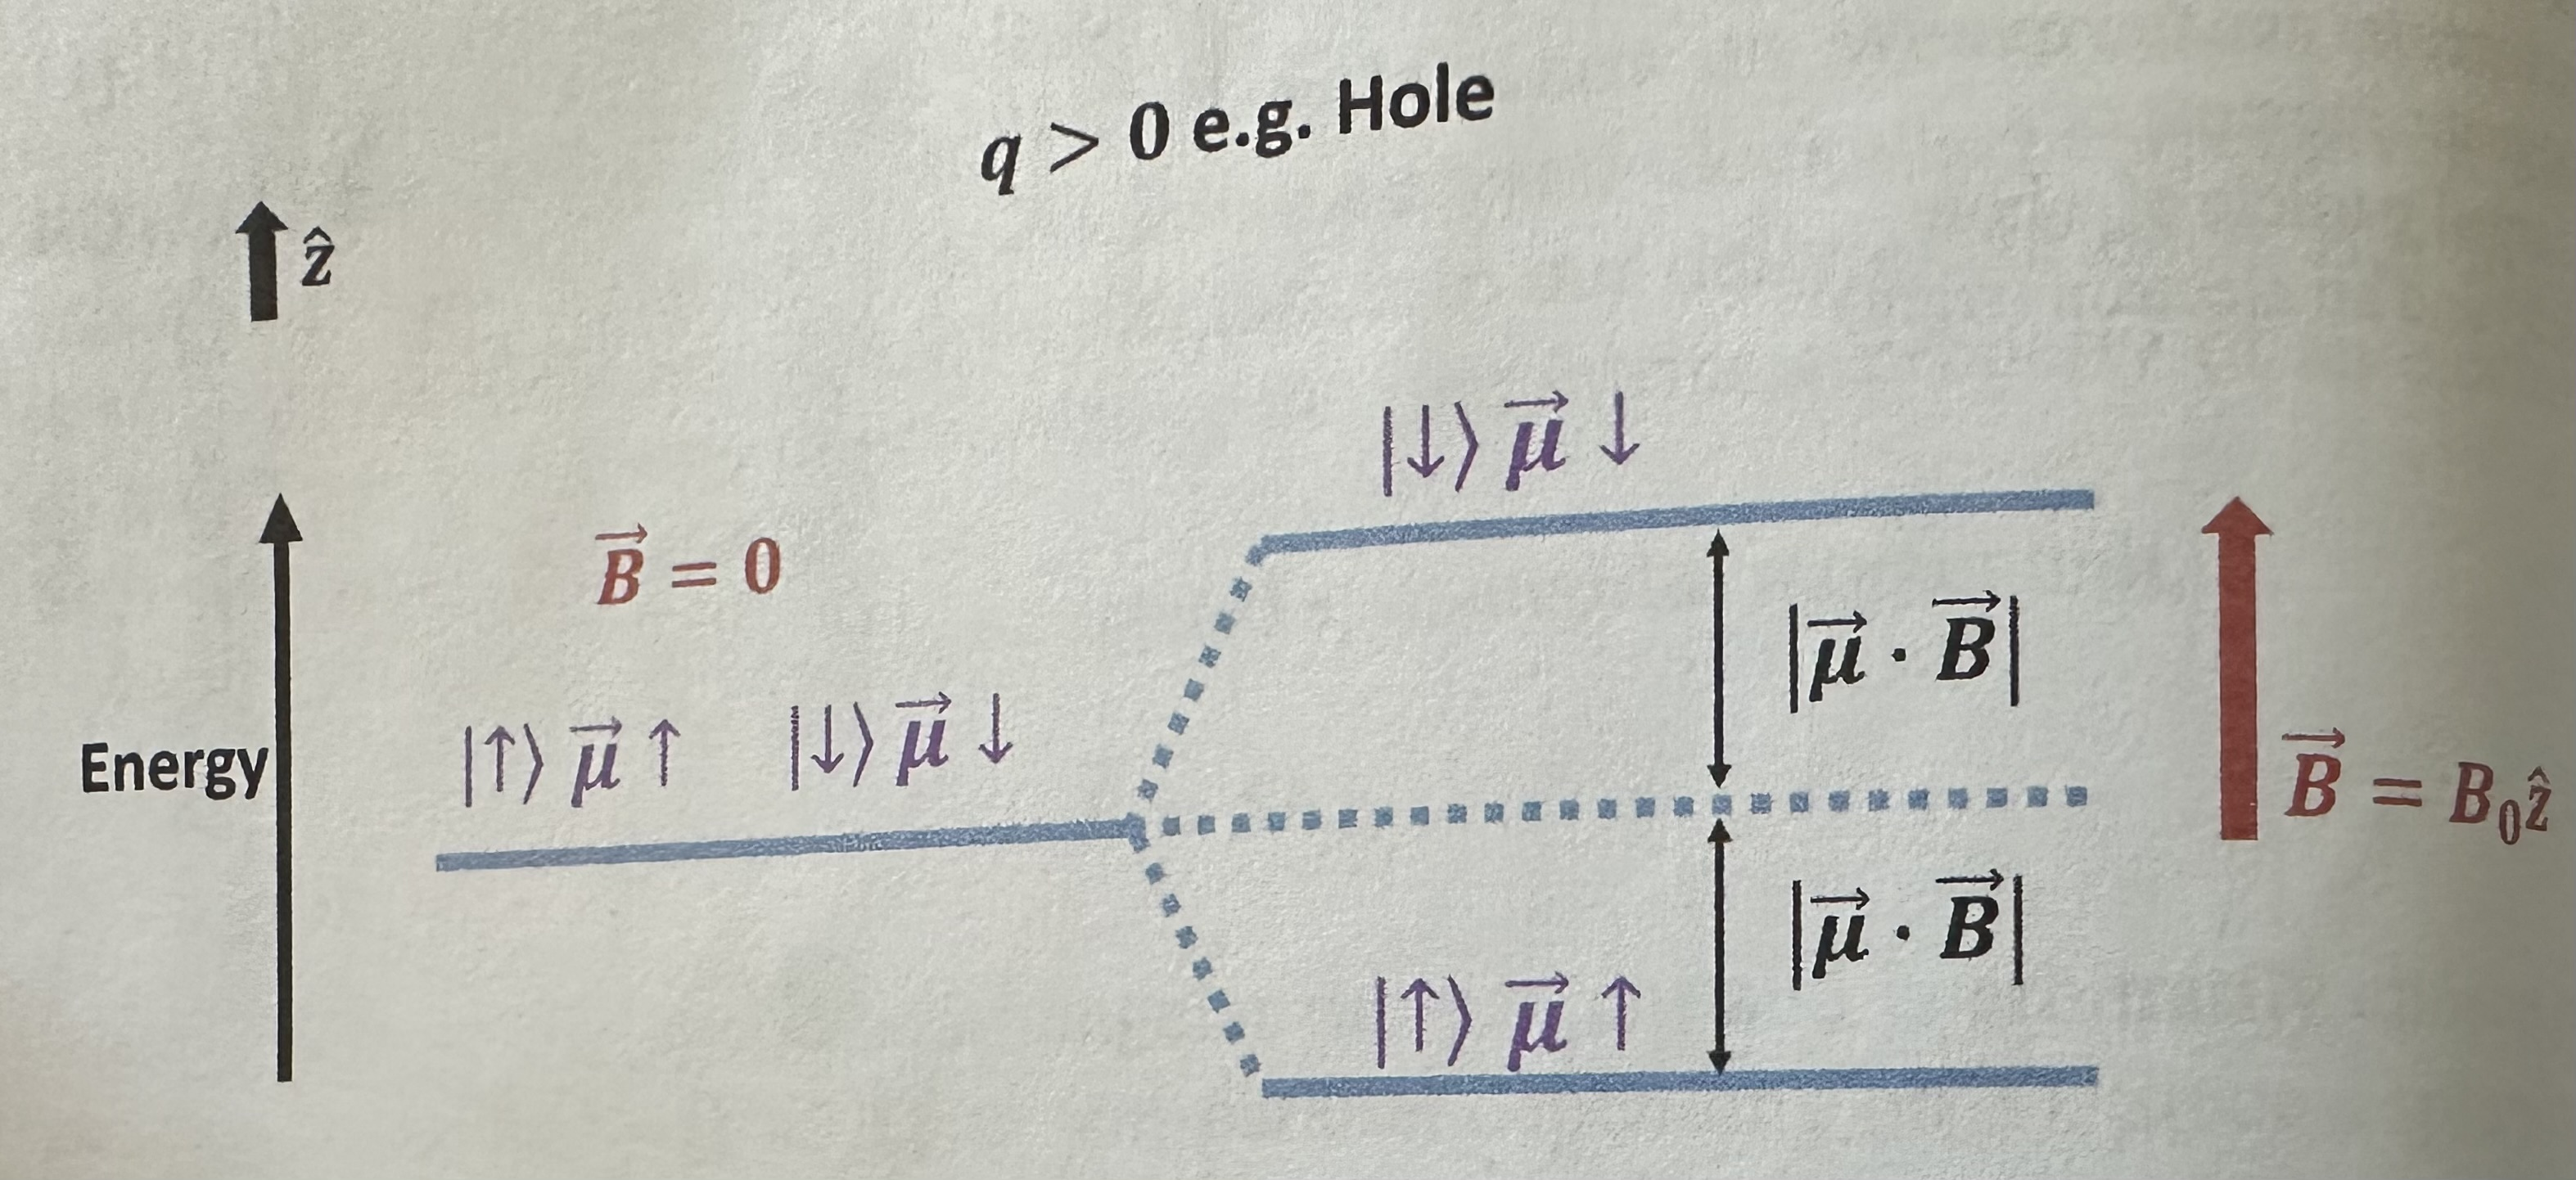
\includegraphics[scale=0.4]{Fig. 7.3.jpeg}\\
\textbf{Fig.7.3} Energy of a positively charged particle with spin under zero (left) or a finite external
magnetic field (right)\\
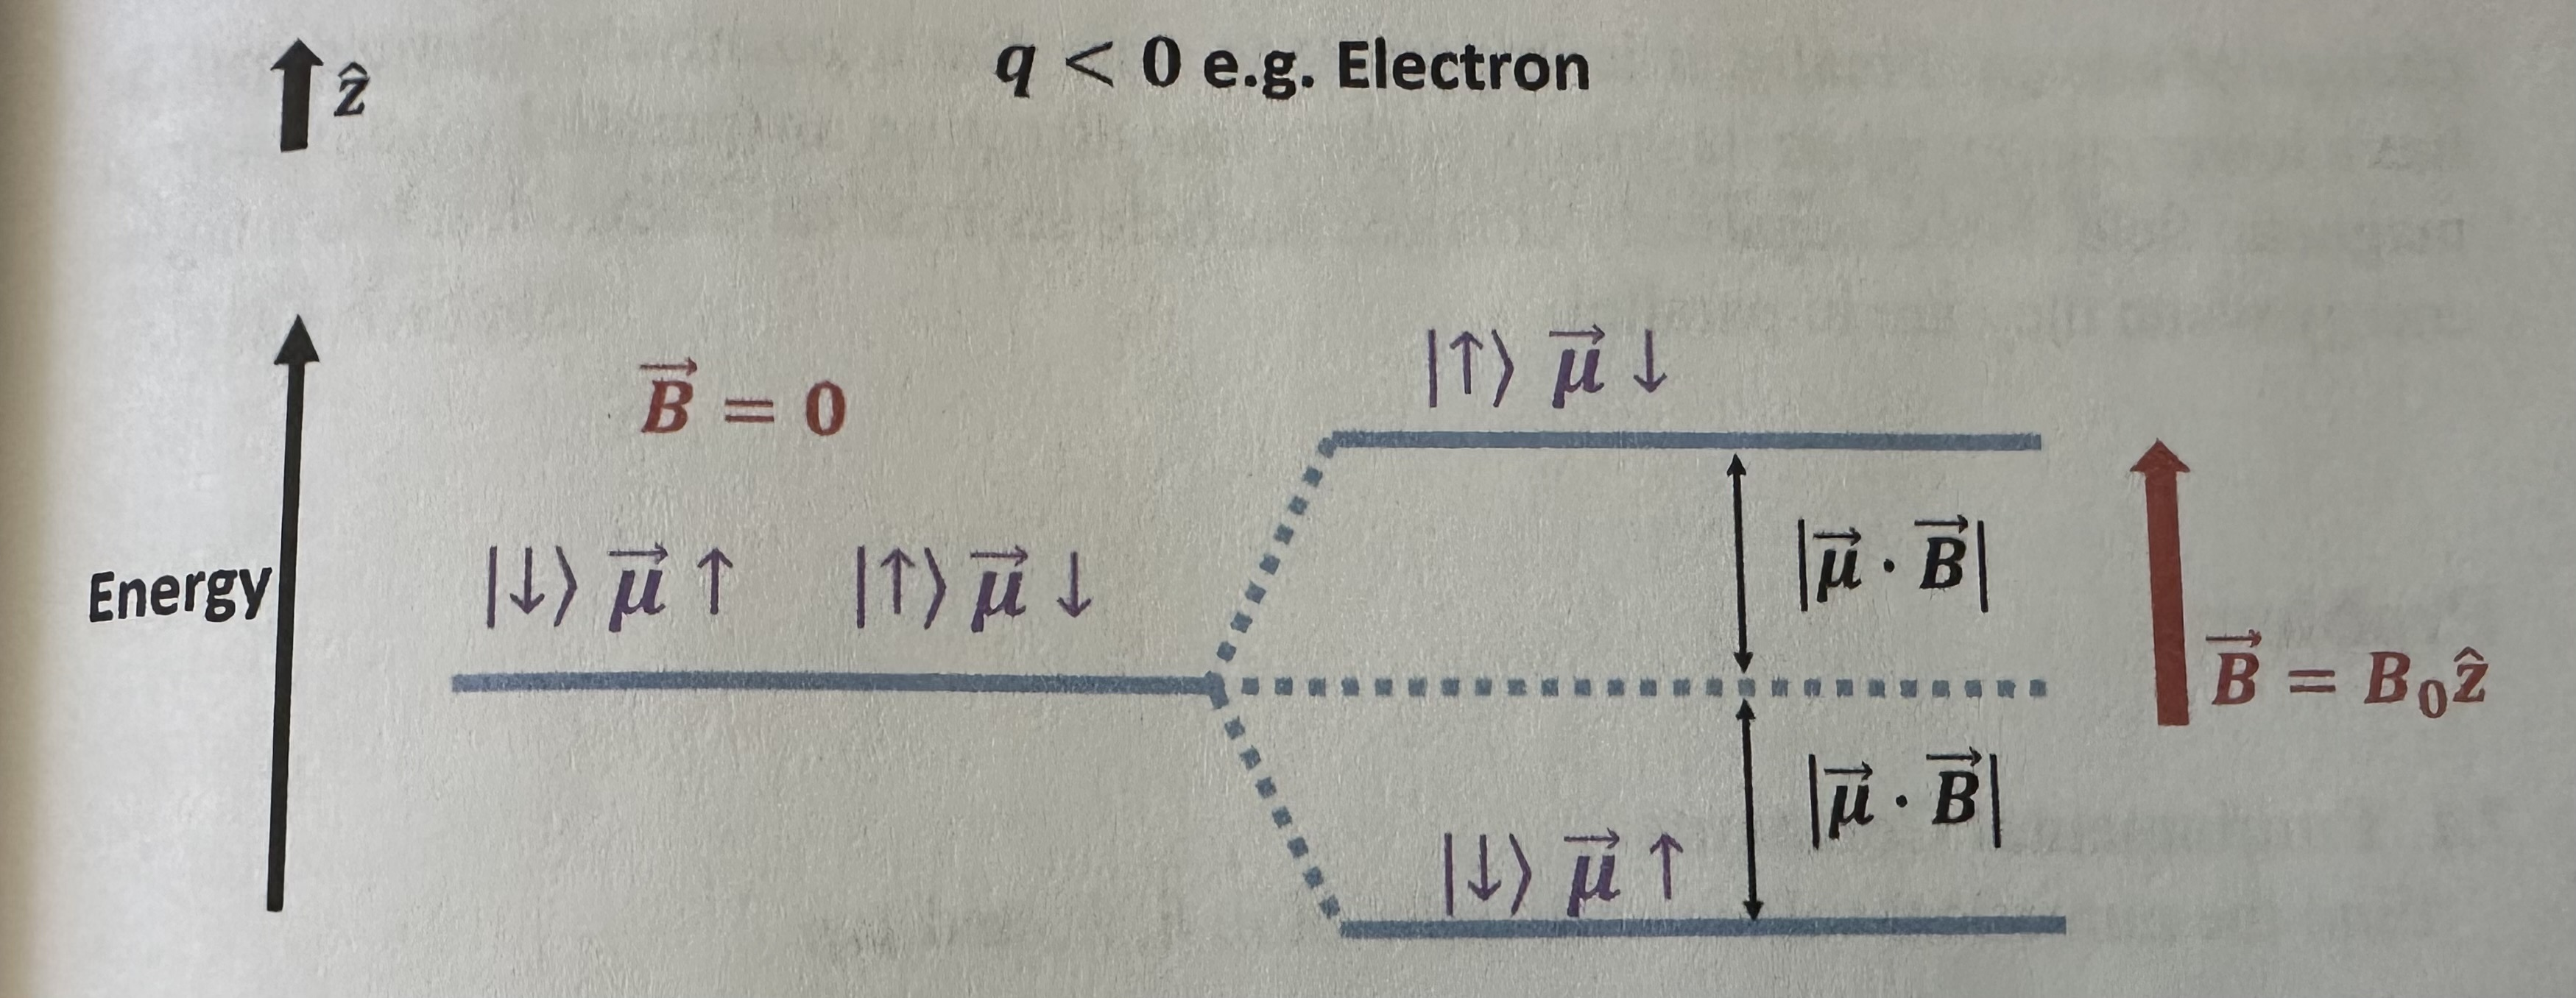
\includegraphics[scale=0.4]{Fig. 7.4.jpeg}\\
\textbf{Fig.7.4} Energy of a negatively charged particle with spin under zero (left) or
a finite external magnetic field (right)\\\\
where $\theta$ is the angle between $\vec{B}$ and $\vec{\mu}$. We also called the change of energy $H$
because this is also the \textbf{interaction Hamiltonian} between the spin magnetic moment and the external magenetic
field. This is a \textbf{dot/inner/scalar product} formula and the result is a scalar
(energy). If $\vec{B}$ and $\vec{\mu}$ are in the same direction (parallel), $\theta=0^\text{o}$
and it has a lower energy ($H=-|\vec{B}||\vec{\mu}|<0$). If $\vec{B}$ and $\vec{\mu}$ are in the 
opposite direection (anti-parallel), $\theta=180^{\text{o}}$ and it has a higher energy
($H=|\vec{B}||\vec{\mu}|>0$) (right of Fig.7.3).

In quantum computing, we use the spin quantum number ($S$ or $\ket{\downarrow}/\ket{\uparrow}$)
more often thatn the spin magentic moment, $\vec{\mu}$. As discussed in the previous
section and Fig.7.2. for a positively charged particle, its spin has the same direction as the spin
magnetic moment. Therefore, for a positively charged particle, when the spin is parallel (anti-parallel)
to the external magnetic field, it has a lower (higher) energy as shown in Fig. 7.3. This is the case
for a hole.

For a negatively charged particel such as an electron, the result is
the opposite. When the spin is parallel (anti-parallel) to the external magnetic
field, it has a higher (lower) energy as shown in Fig.7.4.\\\\\\
\textbf{\large 7.5 Summary}\\\\
Spin is an intrinsic property of elementary particles. From now on, we will only discuss
electrons and holes which are spin-half particles. They have two possible spin values,
$S=\pm \frac{1}{2}$. Like the classical  case that a moving charged particel with 
an angular momentum has a magnetic moment, a charged particle with spin also
has the associated spin angular momentum and spin magnetic moment. As a result,
a charged particle with spin interacts with an external magnetic field resulting in a
change of energy. Finally, it is important to note that a positively charged particle has a
lower energy when its spin is in the same direction as (parallel to) the external
magnetic field. For a negatively charged particle such as an electron, it has a higher energy when
ehty are in parallel.\\\\\\
\textbf{\large Problems}\\\\
\textbf{7.1 Fundamental Constant}

Find the numerical values with units of $e,h,\hbar,$ and $\mu_B$.\\\\
\textbf{7.2 Fundamental Constant}

Calculate the $\gamma$ of electron and hole. What are the masses we should use?

\end{document}
